		\ifx \allfiles \undefined		%编译PPT时注释该行
\documentclass{book}
%%%%%%%%%%%%%%%%%%%%%%%%%%%%%%%%%%%%%%%%%
% 模板資訊:
% 模板名稱:Beamer
% 版本:1.0 (2023.07.09)
% 修改者:Ernie
% 編譯器:XeLaTeX
%
% 原始模板的資訊:
% 模板名稱:Beamer Presentation
% 作者:Vel (vel@latextemplates.com)
% 編譯器:XeLaTeX
% 授權:CC BY-NC-SA 4.0 (https://creativecommons.org/licenses/by-nc-sa/4.0/)
% 下載連結:https://www.LaTeXTemplates.com
%
% 製作本模板之目的:
% 為了讓 LaTeX 初學者能夠輕鬆地完成專業的學術簡報,因此我針對 Vel 製作的模板做了大幅度的修改及附上清楚明瞭的註解。
%
% 如果您有任何問題,可以透過 Email 聯繫我們:stateconlab@gmail.com
% 
% p.s. 也別忘了關注我們的 YouTube、IG 和 Medium 喔!
% 1. YouTube:https://www.youtube.com/@StatEconLab
% 2. IG:https://www.instagram.com/stateconlab
% 3. Mediun:https://medium.com/@stateconlab
%%%%%%%%%%%%%%%%%%%%%%%%%%%%%%%%%%%%%%%%%

%----------------------------------------------------------------------------------------
%	封包與文檔配置
%----------------------------------------------------------------------------------------

\usepackage[space,noindent]{ctex}

% 自訂字體顏色的封包
\usepackage{xcolor} 

%% 自訂顏色

\definecolor{pbblue}{HTML}{0A75A8}% color for the progress bar and the circle
% 數學工具及符號
%\usepackage{mathtools, amsmath, amsfonts, amsthm, latexsym} 

% 分別將數學符號間的間隔加大及加粗
%\usepackage{newtxtext,newtxmath}

% 圖表自動編號的封包
%\usepackage{caption} 

%% 設定自動編號
%\setbeamertemplate{caption}[numbered]

%% 設定圖表編號及標籤的字體大小及字形
%\captionsetup[figure]{font=small, labelfont=md}
%\captionsetup[table]{font=small, labelfont=md}

% 導入圖形與表格的封包
%\usepackage{graphicx}  % \scalebox{} 可用於將過大的表格縮小
%\usepackage{booktabs}

% 排列多個子圖形的封包
%\usepackage{subfigure} 

% 允許表格的一格能多列呈現的封包
%\usepackage{multirow} 

% 可指定表格排版的封包
%\usepackage{array}

% 翻轉表格的封包
%\usepackage{lscape} 

% 序列標號
%\usepackage{enumerate} 

% 繪圖封包 (用於添加浮水印)
\usepackage{tikz}

% 引注參考資料
%\usepackage{natbib}

% 註釋掉大部分的封包
%\usepackage{comment}

\usetikzlibrary{shapes,fit,calc,positioning}

% 設定中文的標籤
%\renewcommand{\figurename}{圖} 
\renewcommand{\tablename}{表} 

%----------------------------------------------------------------------------------------
%	排版形式 (擇一,不選等同選擇默認的排版形式)
%----------------------------------------------------------------------------------------

%\mode<presentation>{
%\usetheme{default}
%\usetheme{AnnArbor}
%\usetheme{Antibes}
%\usetheme{Bergen}
%\usetheme{Berkeley}%演示主题为侧边导航条
%\usetheme{Berlin}
\usetheme{Boadilla}%蓝色主题
%\usetheme{CambridgeUS}
%\usetheme{Copenhagen}
%\usetheme{Darmstadt}
%\usetheme{Dresden}
%\usetheme{Frankfurt}
%\usetheme{Goettingen}
%\usetheme{Hannover}
%\usetheme{Ilmenau}
%\usetheme{JuanLesPins}
%\usetheme{Luebeck}
%\usetheme{Madrid}
%\usetheme{Malmoe}
%\usetheme{Marburg}
%\usetheme{Montpellier}
%\usetheme{PaloAlto}
%\usetheme{Pittsburgh}
%\usetheme{Rochester}
%\usetheme{Singapore}
%\usetheme{Szeged}
%\usetheme{Warsaw}

%----------------------------------------------------------------------------------------
%	外框形式 (擇一,不選等同選擇默認的外框形式)
%----------------------------------------------------------------------------------------

%\useoutertheme{default}
%\useoutertheme{infolines}
%\useoutertheme{miniframes}
%\useoutertheme{smoothbars}
%\useoutertheme{sidebar}
%\useoutertheme{split}
%\useoutertheme{shadow}
%\useoutertheme{tree}
%\useoutertheme{smoothtree}

%----------------------------------------------------------------------------------------
%	外框的自訂義調整 
%----------------------------------------------------------------------------------------

% 外框上緣的字 (fg) 為黑色,背景 (bg) 為白色。
%\setbeamercolor{section in head/foot}{fg=white, bg=black} 

% 外框上緣顯示的章節(section)頁數標籤是否關閉
%\setbeamertemplate{mini frames}{}   

% 調整外框形式的字體大小
%\setbeamerfont{headline}{size=\scriptsize}
%\setbeamerfont{footline}{size=\scriptsize}

% 取消右下方的跳轉工具列
\setbeamertemplate{navigation symbols}{} 

%% 自定義1:外框下緣僅出現名字及頁碼
%\setbeamertemplate{footline}
%{\leavevmode%
%\hbox{%
%\begin{beamercolorbox}[wd=0.5\paperwidth,ht=3ex,dp=1ex,leftskip=2ex]%
%{author in head/foot}%
%{\footnotesize\textbf{\insertshortauthor}}%
%\end{beamercolorbox}%
%\begin{beamercolorbox}[wd=0.5\paperwidth,ht=3ex,dp=1ex,right]%
%{author in head/foot}%
%\footnotesize \textbf{{\insertframenumber{} / \inserttotalframenumber\hspace*{2ex}}} %頁碼控制選項
%\end{beamercolorbox}%
%}}

%% 自定義2:清除外框下緣但僅出頁碼
%\setbeamertemplate{footline}[page number] 

%% 自定義3:清除外框下緣
%\setbeamertemplate{footline}[] 

%----------------------------------------------------------------------------------------
%	顏色主題 (擇一,不選等同選擇默認的顏色主題)
%----------------------------------------------------------------------------------------

%\usecolortheme{default}
%\usecolortheme{albatross}
%\usecolortheme{beaver}
%\usecolortheme{beetle}
%\usecolortheme{crane}
%\usecolortheme{dolphin}
%\usecolortheme{dove}
%\usecolortheme{fly}
%\usecolortheme{lily}
%\usecolortheme{orchid}
%\usecolortheme{rose}
%\usecolortheme{seagull}
%\usecolortheme{seahorse}
\usecolortheme{whale}%颜色主题为
%\usecolortheme{wolverine}

%----------------------------------------------------------------------------------------
%	顏色主題的自訂義調整 
%----------------------------------------------------------------------------------------

% 全文的主題色 (可以特別針對報告對象或機構的代表色調整!)
%\setbeamercolor{structure}{fg=Myblue} 

% 封面頁中標題區塊的底色及字體顏色
%\setbeamercolor{title}{bg=green, fg=black} 

% 各頁標題區塊的底色及字體顏色
%\setbeamercolor{frametitle}{bg=white,fg=black} 

% 全文的內文顏色
%\setbeamercolor{normal text}{fg=orange}

% 數學區塊的標題顏色 
%\setbeamercolor{block title}{bg=blue,fg=yellow} 

% 數學區塊的內文顏色 
%\setbeamercolor{block body}{bg=green,fg=red} 

% 警示文字的顏色
%\setbeamercolor{alerted text}{fg=red} 

%----------------------------------------------------------------------------------------
%	enumerate 及 item 的形狀
%----------------------------------------------------------------------------------------

%\useinnertheme{rounded} % 圓球 (3D)
%\useinnertheme{circles} % 圓形 (2D)
%\useinnertheme{rectangles} % 方形
%\useinnertheme{triangle} % 三角形
%\useinnertheme{inmargin} % 插入邊沿
%\setbeamertemplate{itemize items}[triangle]

%----------------------------------------------------------------------------------------
%	自訂 item 的顏色
%----------------------------------------------------------------------------------------

%\setbeamercolor{item projected}{bg=red}

%----------------------------------------------------------------------------------------
%	個人化的設置及細節調整
%----------------------------------------------------------------------------------------

% 設定頁面邊界
%\setbeamersize{text margin left=0.6cm, text margin right=0.6cm}
%\special{papersize=\the\paperwidth,\the\paperheight}
%\providecommand{\tabularnewline}{\\}
%}

%----------------------------------------------------------------------------------------
%	個人化的背景調控
%----------------------------------------------------------------------------------------

% 背景照片設置
%\setbeamertemplate{background}{\includegraphics[height=\paperheight]{Fig/Background.png}}

% 浮水印設定
%\usebackgroundtemplate{%
%	\tikz[overlay, remember picture] % 讓 logo 能每頁都顯示
%	\node[opacity=0.3, below=-1.25cm, at=(current page.center)] % 調整透明度 (opacity) 及浮水印的位置
%	{\includegraphics[scale = 0.14]{Fig/nthulogo.png}}; % 載入 logo 及調整大小
%	}

\begin{document}
		\else						%编译PPT时注释该行
		%\newpage
		\fi						%编译PPT时注释该行
\watermark{50}{9}{热工班组}
\chapter[2024年09月份技术培训考试]{	\hspace*{-0.3em}\biaoti{2024}{09}{热工专业}}
姓名:\uline{ \ \  \  \ \ \ \ \ \ \ \ \ \ \ \ \ \ }\hfill 得分:\uline{ \ \  \  \ \ \ \ \ \  \ \ \ \ \ \ }
%\zysx
\section{\xzt{5}{2}{10}}
\begin{enumerate}
\item 我厂脱硫净烟气CEMS二氧化硫和氮氧化物分析仪采用\xz{A}测量方法。
\xx{稀释法}{抽取式}{激光后散射法}{等速采样}
\item 我厂脱硫净烟气CEMS二氧化硫分析仪测量原理为\xz{B}。
\xx{化学发光原理}{脉冲荧光法原理}{激光后散射法}{NRIR不分光红外法}
\item 我厂脱硫净烟气CEMS氮氧化物分析仪测量原理为\xz{A}。
\xx{化学发光原理}{脉冲荧光法原理}{激光后散射法}{NRIR不分光红外法}
\item 我厂脱硫净烟气在线粉尘烟度计测量原理为\xz{B}。
\xx{NRIR不分光红外法}{光散射法}{脉冲荧光法原理}{静电技术}
\item 我厂净烟气粉尘探头控制器内流量计不包含以下哪种流量计\xz{A}。
\xx{喷嘴流量计}{稀释气流量计}{旁路气流量计}{样气流量计}
\end{enumerate}
\section{\tkt{4}{2}{30}}
\begin{enumerate}
	\setcounter{enumi}{5}
	\item CEMS响应时间包括\tk[2.5]{仪表响应时间}和\tk[2.5]{系统响应时间},分别要求响应时间小于等于\tk{120s}和小于等于\tk{200s}。
\item 我厂净烟气CEMS数据包含\tk[2]{二氧化硫}、\tk[2]{氮氧化物}、\tk[2]{氧气}、\tk[2]{粉尘}、\tk[2]{温度}、\tk[2]{压力}、\tk[2]{流速}、\tk[2]{湿度}。
	\item 我厂净烟气MODEL 200稀释法CEMS设备中音速小孔的稀释比为\tk{100:1}。
\item 我厂净烟气粉尘,SO2,NOX折算时,如果氧量值大于6\%,则折算值\tk{大于}干基值,干基值是指烟气经预处理,露点温度小于等于\tk{4}℃时,烟气中各污染物的浓度。
\end{enumerate}
\section{\stt{40}}
\begin{enumerate}
	\setcounter{enumi}{9}
	\item CEMS仪表响应时间指的是什么?\fenzhi{5}
\wdt[3]{答:仪表响应时间指从观察到分析仪示值产生一个阶跃增加或阶跃减少的时刻起,到其示值达到标准气体标称值90\%或10\%的时刻止,中间的时间间隔。}\\
	\item CEMS系统响应时间指的是什么?\fenzhi{5}
\wdt[3]{答:系统响应时间指从CEMS系统采样探头通入标准气体的时刻起,到分析仪示值达到标准气体标称值90\%的时刻止,中间的时间间隔。包括管线传输时间和仪表响应时间。}\\
%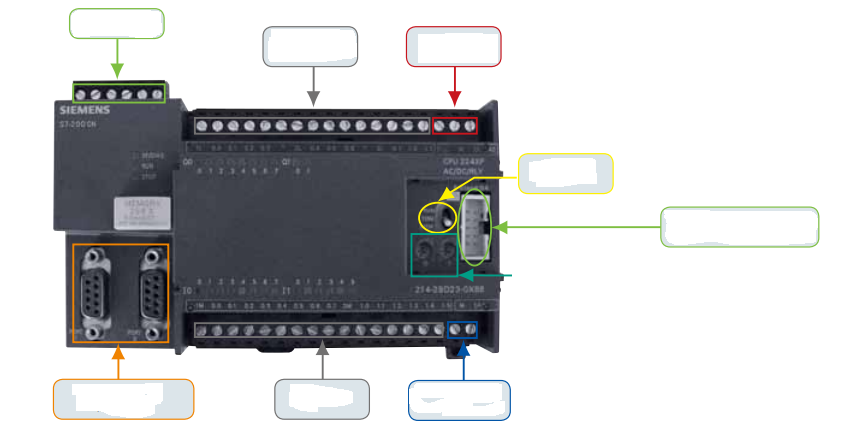
\includegraphics[angle=0,width=500pt,trim=0 0 0 0,clip]{picture/200plc.png}%答案需要替换下图片
%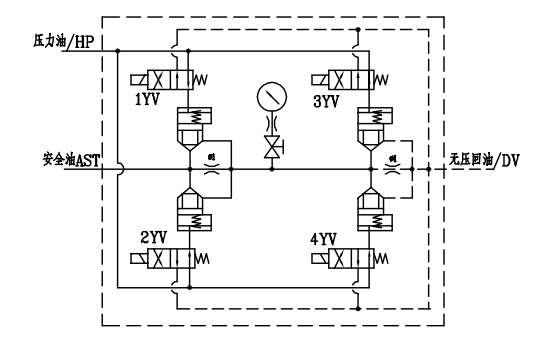
\includegraphics[angle=0,width=500pt,trim=0 0 0 0,clip]{picture/AST.png}%带答案图片
\item 在下图中方框中填入各气路名称,并分别标出正常采样状态下各气路方向?\fenzhi{15}
%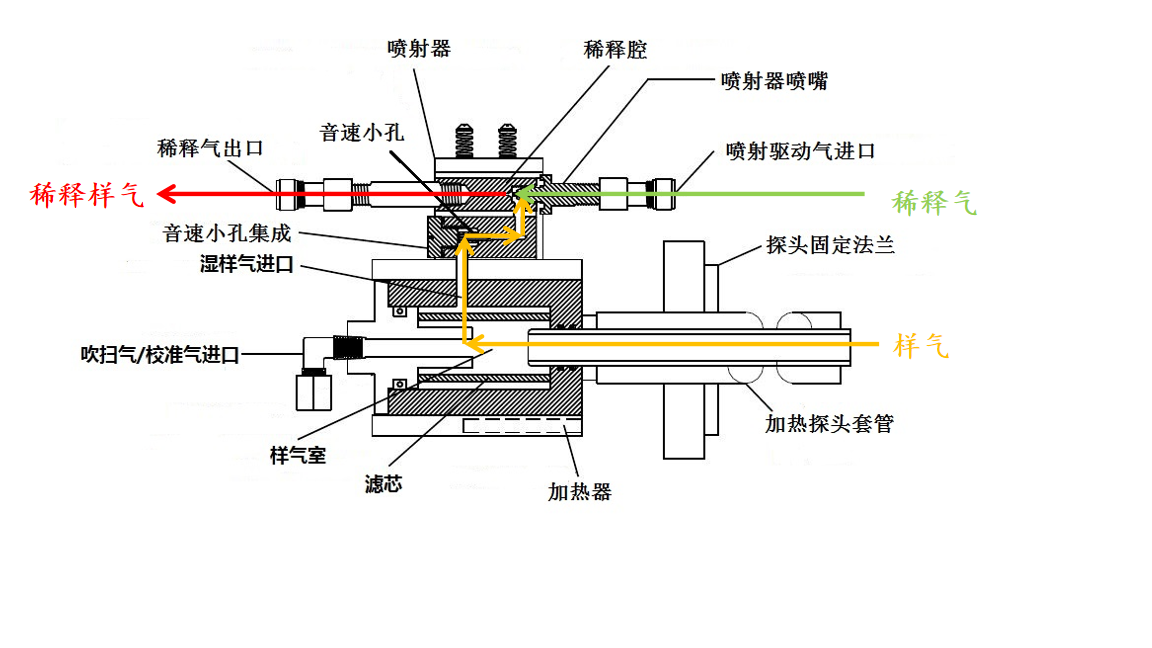
\includegraphics[angle=0,width=450pt,trim=0 0 0 0,clip]{picture/so2_da.png}\\
	%\tupian{picture/so2_da.png}{picture/so2.png}
	\tupian{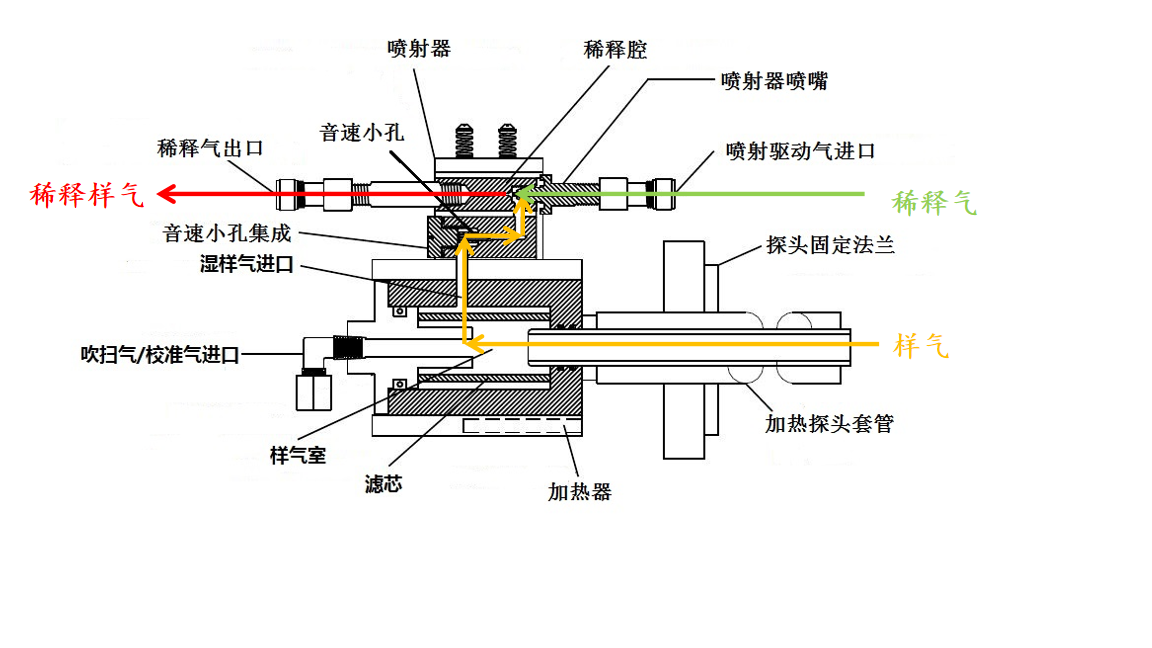
\includegraphics[angle=0,width=450pt,trim=0 0 0 0,clip]{picture/so2_da.png}\\}{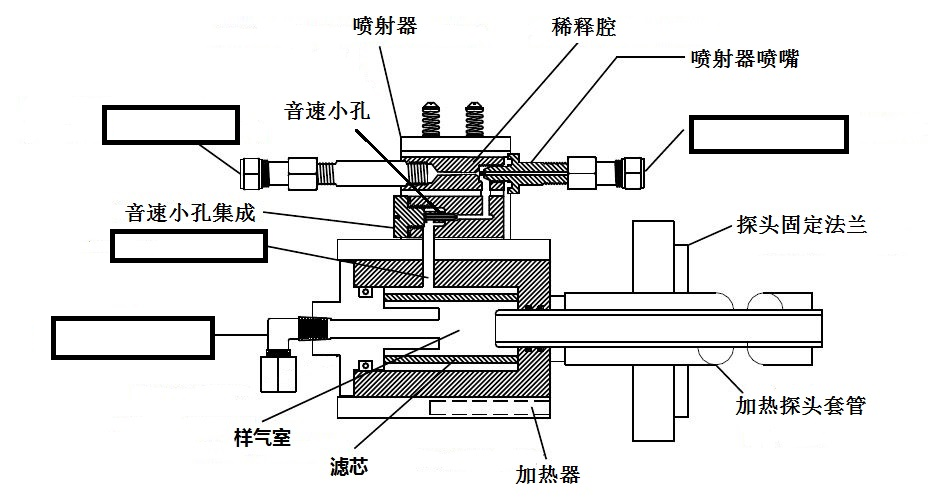
\includegraphics[angle=0,width=450pt,trim=0 0 0 0,clip]{picture/so2.png}\\}
\item 在下图中标出粉尘仪各流量名称及数值?\fenzhi{15}
%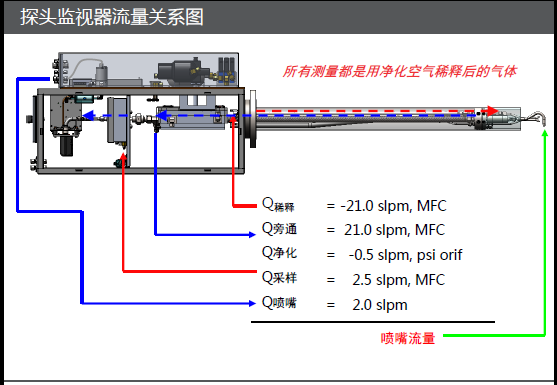
\includegraphics[angle=0,width=450pt,trim=0 0 0 0,clip]{picture/dust_da.png}\\
	\tupian{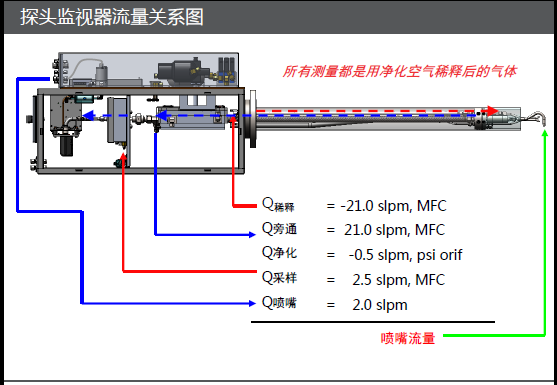
\includegraphics[angle=0,width=450pt,trim=0 0 0 0,clip]{picture/dust_da.png}\\}{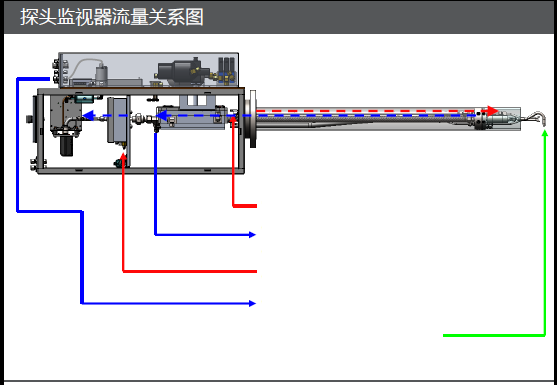
\includegraphics[angle=0,width=450pt,trim=0 0 0 0,clip]{picture/dust.png}\\}
\end{enumerate}
\section{\jdt{20}}
\begin{enumerate}
	\setcounter{enumi}{13}
\item 画出我厂净烟气CEMS各数据电信号分布示意图(标明各数据测量设备的名称,电信号从测量设备最终分别到DCS系统、环保局、CEMS报表系统)\fenzhi{20}
\wdt[6]{答:\\
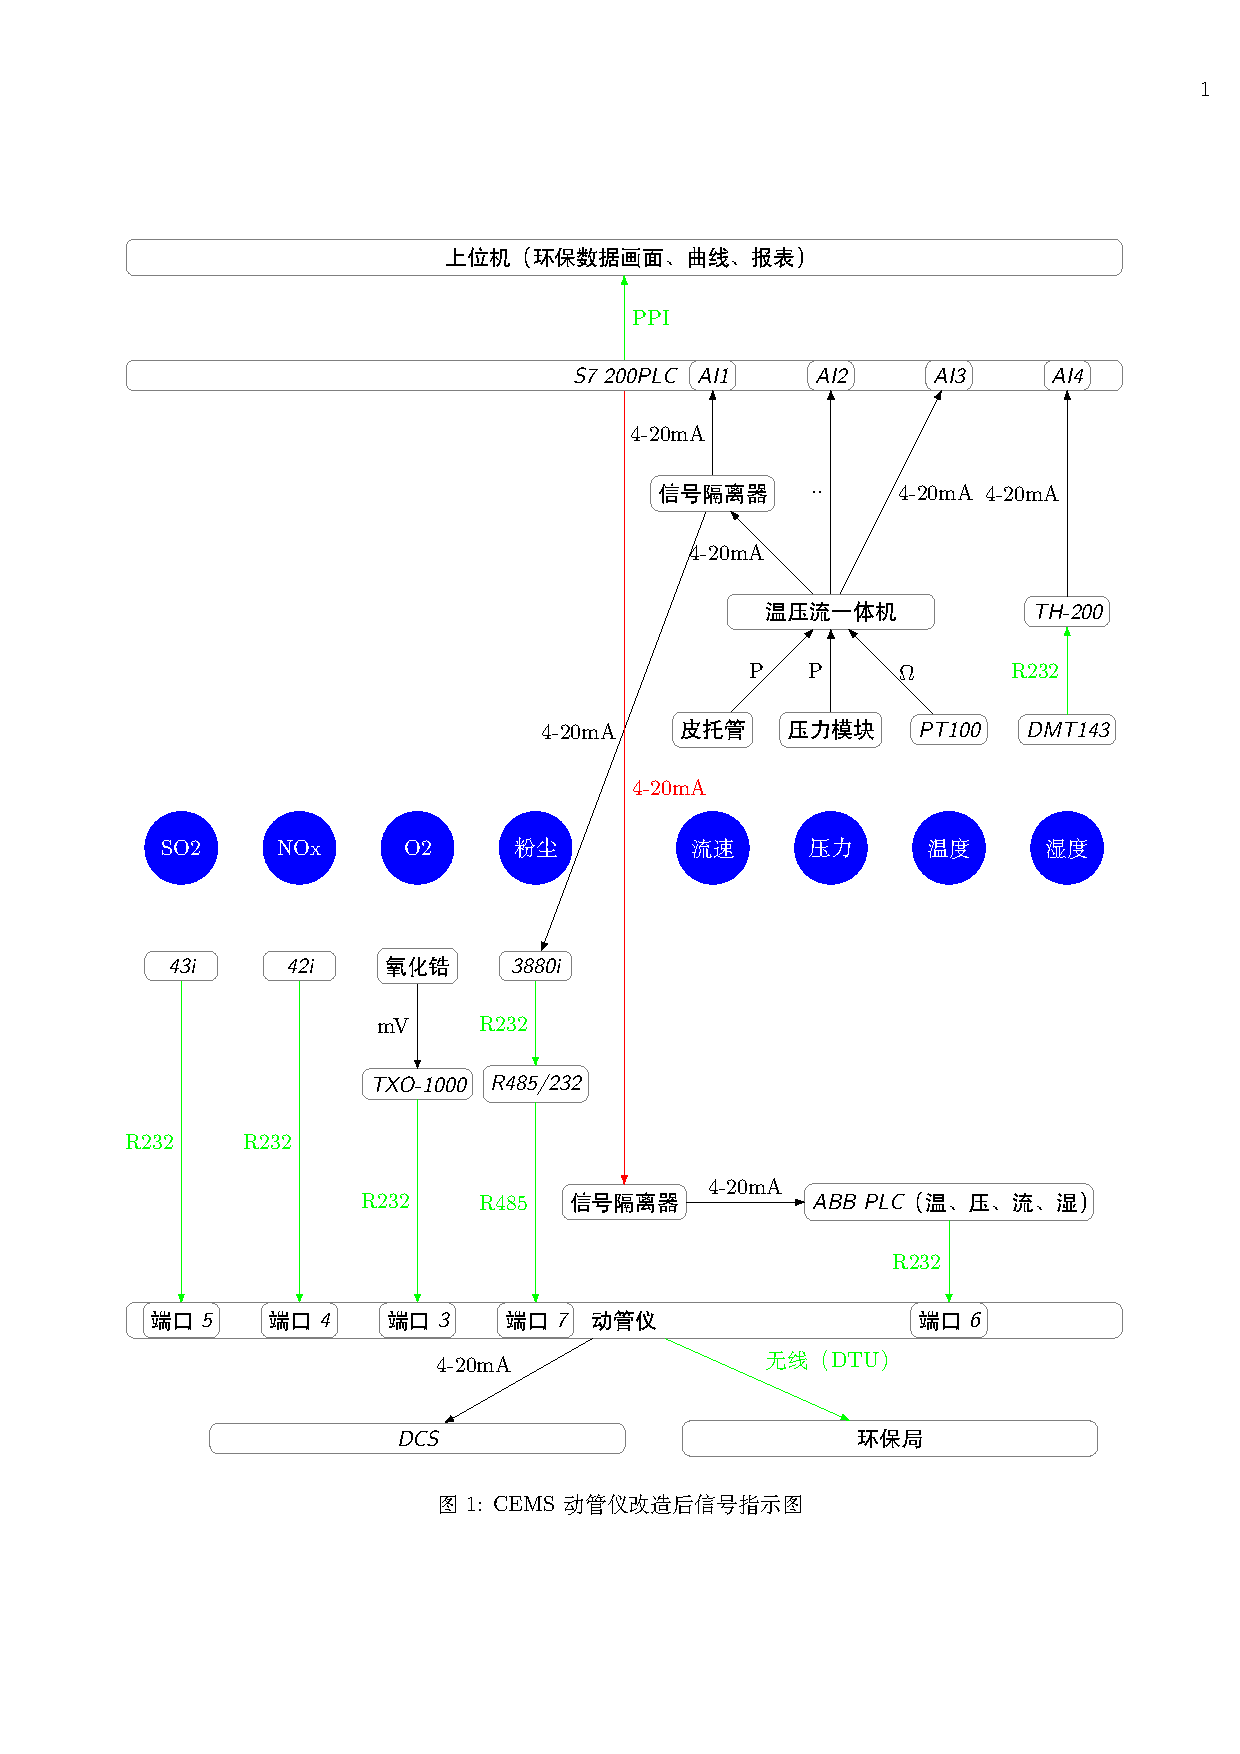
\includegraphics[angle=0,width=500pt,trim=50 0 0 50,clip]{picture/huan.pdf}%带答案图片
}

\end{enumerate}
		\ifx \allfiles \undefined
\end{document}
\fi
